
%(BEGIN_QUESTION)
% Copyright 2011, Tony R. Kuphaldt, released under the Creative Commons Attribution License (v 1.0)
% This means you may do almost anything with this work of mine, so long as you give me proper credit

Suppose we were to inject the same mobile phase into two different columns, each with a different density of stationary phase material (``packing''):

$$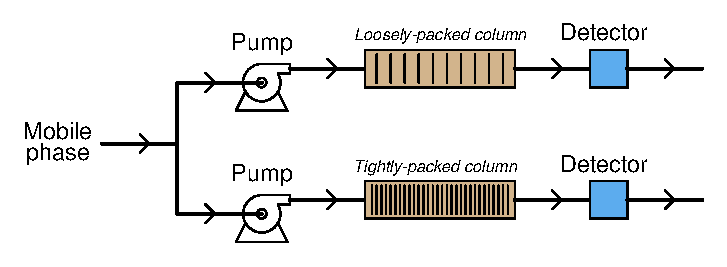
\includegraphics[width=15.5cm]{i00667x01.eps}$$

Assuming all other factors being equal, which column will do a better job separating different components of the mobile phase (i.e. different chemical substances mixed together in the same input sample)?  Which column will do a {\it faster} job separating the components?

\vskip 20pt \vbox{\hrule \hbox{\strut \vrule{} {\bf Suggestions for Socratic discussion} \vrule} \hrule}

\begin{itemize}
\item{} Chromatography is analogous to a marathon race, where groups of runners become further separated over time by their relative speeds.  By the end of the race, it is easy to identify who is fast, who is slow, and how many of each type of runner there was in the starting group at the beginning of the race.  Relate this question of comparing two columns to the analogy of a marathon race: what does a tightly-packed column represent, versus a loosely-packed column?
\item{} An important variable affecting the retention time of a compound inside a chromatograph column is {\it temperature}.  Explain how an increase in column temperature would affect the propagation of a {\it gaseous} compound.  Then, explain how an increase in column temperature would affect the propagation of a {\it liquid} compound.
\item{} Identify other variables affecting the retention time of a compound inside a chromatograph column besides packing density.
\end{itemize}

\underbar{file i00667}
%(END_QUESTION)





%(BEGIN_ANSWER)


%(END_ANSWER)





%(BEGIN_NOTES)

The tightly-packed column will do a better job separating the different components, but it will take longer to do so.

\vskip 10pt

Changes in column temperature affect fluid viscosity.  For gases, increased temperature {\it increases} viscosity, causing the compound to flow slower.  For liquids, increased temperature usually causes {\it decreased} viscosity, causing the compound to flow faster.

%INDEX% Measurement, analytical: chromatography

%(END_NOTES)


